\chapter{Теоретическая часть}
\section{Полупроводник}
Рассматривая полупроводники, мы будем говорить о кристаллических телах. Для анализа таких тел необходимо решить уравнение Шредингера для нахождения, к примеру, энергических уровней. В целях упрощения задачи и сохранения наиболее характерных черт системы в Зонной теории вводится ряд допущений \cite{Kalashnikov}: 
\begin{enumerate}
	\item Атомные ядра являются неподвижными источниками поля, действующего на электроны;
	\item Расположения атомных ядер в пространстве является строго периодичным: они располагаются в узлах идеальной кристаллической решетки;
	\item Взаимодействие электронов друг с другом заменяется некоторым внешним полем.
\end{enumerate}

\begin{lstlisting}[style=pseudocode,caption={Алгоритм оценки дипломных работ}]
def EvaluateDiplomas():
    for each student in Masters:
        student.Mark := 5
    for each student in Engineers:
        if Good(student):
            student.Mark := 5
        else:
            student.Mark := 4
\end{lstlisting}

\subsection{Зонная структура}
В следствии симметрии и периодичности идеального кристалла по различным направлениям и теории Блоха, для описания дисперсии электронов используют зоны Бриллюэна. Так как закон дисперсии периодичен на всем кристалле, для его описания можно использовать только первую зону Бриллюэна. 
\begin{figure}[h]
    \begin{minipage}[b]{0.5\textwidth}
		\centering
	    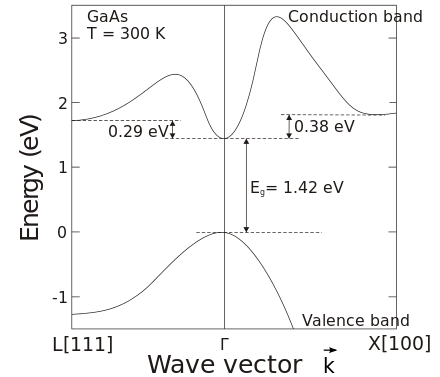
\includegraphics[width=0.9\textwidth]{assets/GaAs_E}
	    \caption{Зонная структура $GaAs$}
	\end{minipage}
	\hfill
	\begin{minipage}[b]{0.45\textwidth}
		\centering
		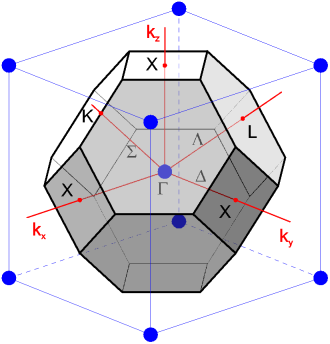
\includegraphics[width=0.8\textwidth]{assets/ZnLaer}
	    \caption{Элементарная ячейка типа Цинковой обманки}
	\end{minipage}
\end{figure}

\subsection{Зонная диаграмма}
Для наглядного представления и сравнения полупроводников и других материалов удобно использовать зонную диаграмму (рис.~\ref{img:Zone}).
\begin{figure}
	\centering
	\includegraphics[width=\textwidth]{assets/Zone}
    \caption{Характерный вид зонной диаграммы для различных материалов}
    \label{img:Zone}
\end{figure}\\
\begin{conditions}
	$E_{c}$ & дно зоны проводимости (ЗП);\\
	$E_{v}$ & потолок валентной зоны (ВЗ);\\
	$E_{F}$ & уровень (квазиуровень) Ферми;\\
	$E_{g}$ & запрещенная зона (ЗЗ);\\
	$\chi$ & электронное сродство;\\
	$\varphi$ & работа выхода.
\end{conditions}
Параметры зонной структуры $Al_{x}Ga_{1−x}As$ приведены в табл.~\ref{tab:AlGaAsBandE} \cite{Shilaev}.
\begin{center}
  \begin{longtable}{|c|c|}
    \caption{Основные параметры $Al_{x}Ga_{1−x}As$}
    \label{tab:AlGaAsBandE}
    \\ \hline
    Параметр & $Al_{x}Ga_{1−x}As$ \\
    \hline \endfirsthead
    \subcaption{Продолжение таблицы~\ref{tab:AlGaAsBandE}}
    \\ \hline \endhead
    \hline \subcaption{Продолжение на след. стр.}
    \endfoot
    \hline \endlastfoot
	Кристаллическая структура& Типа цинковой обманки \\ \hline
	Постоянная решетки $a[nm]$  & $0.56533+0.00078x$ \\ \hline
	$E_{g}^{\Gamma}[eV],\, x < 0.45$    & $1.424+1.247x$ \\ \hline
	$E_{g}^{\Gamma}[eV],\, x > 0.45$    & $1.656+0.215x+0.143x^{2}$ \\ \hline
	% $\Delta E_{c}^{\Gamma}[eV],\, x < 0.45$    & $0.773x$ \\ \hline
	% $\Delta E_{c}^{\Gamma}[eV],\, x > 0.45$    & $0.232-0.259x+1.147x^{2}$ \\ \hline
	$m_{e}^{\Gamma}$    & $0.067+0.083x$ \\ \hline
	$m_{lh}$    & $0.082+0.071x$ \\ \hline
	$N_{atoms}[1/sm^{-3}]$    & $(4.42-0.17x)10^{22}$
  \end{longtable}
\end{center}

\subsection{Плотность состояний}
Для вычисления числа электронов в зоне проводимости (ЗП) необходимо знать количество разрешенных состояний в ЗП. Для этого рассмотрим фазовое пространство, в котором объем $V_{\text{фаз}}$ занимаемый одним электроном \cite{Shinkarenko}:
\begin{gather}
	\label{eq:Vphaz}
 	V_{\text{фаз}} = V_{xyz}V_{p_{x}p_{y}p_{z}};\\
	\label{eq:Vxyz}
 	V_{xyz} = xyz;\\
 	\label{eq:Vp}
 	V_{p_{x}p_{y}p_{z}} = \frac{4}{3}\pi p^{3};\\
 	\label{eq:p}
 	p = \sqrt{2mE},
\end{gather} 
\begin{conditions}
	$V_{xyz}$ & объем в координатном пространстве;\\
	$V_{p_{x}p_{y}p_{z}}$ & объем в импульсном пространстве. 
\end{conditions}
Согласно закону Гейзенберга:
\begin{equation}
	\label{eq:gez}
	\Delta p_{x} \Delta x \geq h,
\end{equation}
\begin{conditions}
	$h$ & постоянная Планка.
\end{conditions}
Тогда для трехмерного движения неопределенность составит:
\begin{equation}
	\label{eq:gez3D}
	\Delta p_{x} \Delta x \Delta p_{y} \Delta y\Delta p_{z} \Delta z\geq h^{3}
\end{equation}
Из (\ref{eq:Vphaz}), (\ref{eq:Vxyz}), (\ref{eq:Vp}), (\ref{eq:gez3D}) получим полное число электронов ($N(p)$) в единичном объеме:
\begin{gather}
	N(p) = 2* \frac{V_{\text{фаз}}}{V_{xyz}h^{3}} = \frac{8\pi p^{3}}{3h^{3}} \Rightarrow \\
	\Rightarrow N(E) =  \frac{8\pi (2mE)^{3/2}}{3h^{3}}.
\end{gather}
Двойка появилась из-за того, что электрон имеет квантовое спиновое число равное $\pm 1/2$, и два электрона с разным спином могут занимать одно состояние.

Плотность разрешённых состояний ($g(E)$)~--- число электронов в единице объёма с энергией $E$, приходящихся на единичный интервал энергии. По определению:
\begin{gather}
	g(E) = \frac{d}{dE}\,N(E) = \frac{4\pi (2m)^{3/2}}{h^{2}}\sqrt{E}.
\end{gather}


\subsection{Концентрация носителей заряда}
Так как электроны имеют полуцелый спин (фермионы)~--- они подчиняются статистике Ферми-Дирака:
\begin{equation}
	f(E) = \frac{1}{1 + e^{\frac{E-E_{F}}{k_{B}T}}},
\end{equation}
\begin{conditions}
	$E$ & энергия электрона;\\
	$E_{F}$ & уровень Ферми;\\
	$k_B$ & постоянная Больцмана;\\
	$T$ & температура;\\
	$k_{B}T$ & <<опорный>> потенциал.
\end{conditions}
Физический смысл статистики Ферми-Дирака: вероятность электрона иметь энергию равную $E$.
\begin{figure}
	\centering
	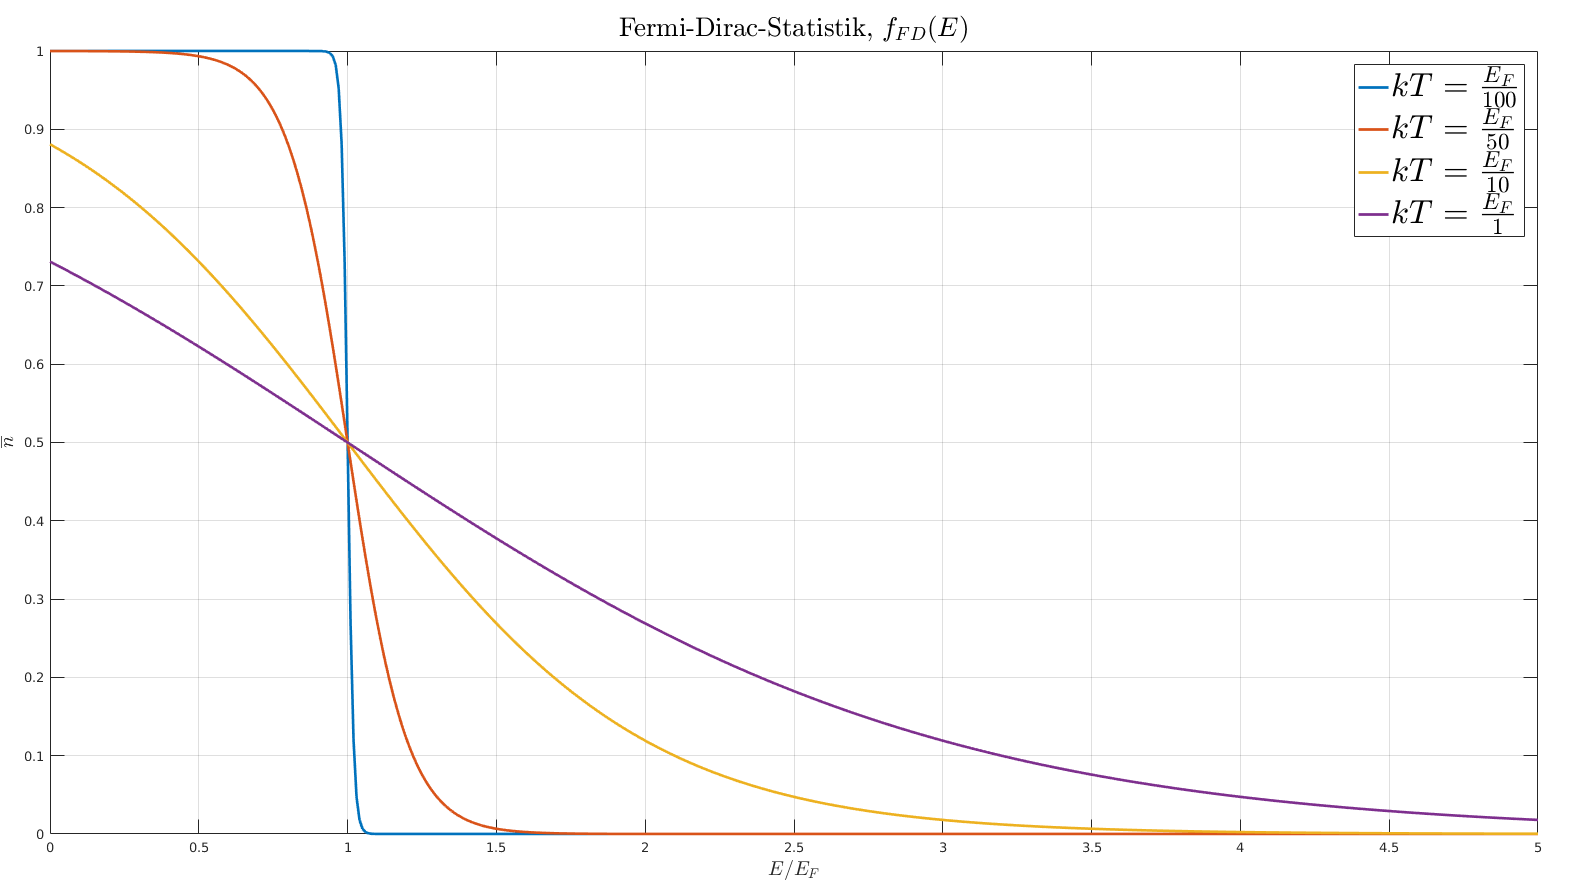
\includegraphics[width=0.99\textwidth]{assets/FD}
    \caption{Статистика Ферми-Дирака}
    \label{img:FD}
\end{figure}

Концентрацию электронов ($n$) зависит от плотности состояний ($g(E)$) в ЗП и функции распределения электронов по энергиям ($f(E)$):
\begin{gather}
	\label{eq:n}
	n = \int\limits_{0}^{+\infty}\! g(E)f(E) \,dE =  \frac{2^{1/2}m^{3/2}}{\pi^{2}\hbar^{3}}\int\limits_{0}^{+\infty}\! \frac{\sqrt[]{E}}{e^{\frac{E-\mu}{kT}}+1} \,dE,
\end{gather}
\begin{conditions}
	$\hbar$ & постоянная Дирака.
\end{conditions}
\subsubsection{Собственный полупроводник}
В случаи собственного проводника, когда уровень Ферми лежит в центре ЗЗ, и полупроводник является невырожденным расчет интеграла (\ref{eq:n}) упрощается в приближении идеального электронного газа (Максвелла-Больцмана):
\begin{gather*}
	n =\! \int\limits_{0}^{+\infty}\! g(E)f_{FD}(E) \,dE \approx \!\int\limits_{0}^{+\infty}\! g(E)f_{MB}(E) \,dE =\\
	= \frac{2^{1/2}m^{3/2}}{\pi^{2}\hbar^{3}} e^{-\frac{E_{c} - E_{F}}{k_{B}T}} \int\limits_{0}^{+\infty}\! E^{1/2}e^{-E}dE = \frac{m^{3/2}}{2^{1/2}\pi^{3/2}\hbar^{3}} e^{-\frac{E_{c} - E_{F}}{k_{B}T}};
\end{gather*}
\begin{gather}
	n = N_{c}e^{-\frac{E_{c} - E_{F}}{k_{B}T}};\\
	N_{c} = 2 \bigg( \frac{mk_{B}T}{2\pi \hbar^{2}} \bigg)^{3/2},
\end{gather}
\begin{conditions}
	$N_{c}$ & эффективная плотность состояний в ЗП;\\
	$E_{c}$ & энергия дна ЗП;\\
	$m$ & эффективная масса электрона в ЗП.
\end{conditions}

Проведя аналогичные рассуждения для дырок в ВЗ получим:
\begin{gather}
	p = N_{v}e^{-\frac{E_{F} - E_{v}}{k_{B}T}};\\
	N_{v} = 2 \bigg( \frac{mk_{B}T}{2\pi \hbar^{2}} \bigg)^{3/2},
\end{gather}
\begin{conditions}
	$N_{v}$ & эффективная плотность состояний в ВЗ;\\
	$E_{v}$ & энергия потолка ВЗ;\\
	$m$ & эффективная масса дырки в ВЗ.
\end{conditions}

Так как в чистом (\textit{intrinsic}) полупроводнике количество дырок равно количеству, перемножив обе части получим:
\begin{gather}
	\label{eq:doMass}
	np = n_{i}^{2} = N_{c}N_{v}e^{-\frac{E_{F} - E_{v}}{k_{B}T}}e^{-\frac{E_{c} - E_{F}}{k_{B}T}} = N_{c}N_{v}e^{-\frac{E_{c} - E_{v}}{k_{B}T}};\\
	\label{eq:ni}
	n_{i} = \sqrt{N_{c}N_{v}}e^{-\frac{E_{g}}{2k_{B}T}},
\end{gather}
\begin{conditions}
	$n_{i}$ & концентрация собственных носителей заряда;\\
	$E_{g}$ & ширина ЗЗ;\\
	$N_{v}$ & эффективная плотность состояний в ВЗ;\\
	$N_{c}$ & эффективная плотность состояний в ЗП.
\end{conditions}

Формула (\ref{eq:doMass}) называется <<законом действующий масс>>.

\subsubsection{Легированный полупроводник}
При легировании полупроводника донорной или акцепторной примесью, уровень Ферми подымается к дну ЗП или опускается к потолку ВЗ соответственно.

Если разница между дном ЗП (потолком ВЗ) и уровнем Ферми превышает несколько энергий теплового колебания и уровень Ферми лежит в ЗЗ, то полупроводник невырожденный:
\begin{gather}
 	E_{c} - E_{F} > 3k_{B}T;\\
 	E_{F} - E_{v} > 3k_{B}T.
\end{gather}
Тогда приближенное значение квазиуровня Ферми для невырожденного полупроводника можно рассчитать\cite{Shinkarenko}:
\begin{gather}
	E_{F}^{n} = E_{F}^{i} + k_{B}T\ln\frac{N_{D}}{n_{i}};\\
	E_{F}^{p} = E_{F}^{i} - k_{B}T\ln\frac{N_{A}}{n_{i}},
\end{gather}
\begin{conditions}
	$E_{F}^{n}$ & уровень Ферми невырожденного полупроводника $n$--типа;\\
	$E_{F}^{p}$ & уровень Ферми невырожденного полупроводника $p$--типа;\\
	$E_{F}^{i}$ & уровень Ферми невырожденного полупроводника $i$--типа;
\end{conditions}

Если полупроводник вырожден, положение уровня Ферми находится, как решение уравнения (\ref{eq:n}). Приближенное положение уровня Ферми можно найти\cite{Kalashnikov}:
\begin{gather}
	\label{eq:EFn+}
	E_{F}^{n} = \frac{(3\pi^{2}N_{D})^{2/3}\hbar^{2}}{2m};\\
	E_{F}^{p} = \frac{(3\pi^{2}N_{A})^{2/3}\hbar^{2}}{2m},
\end{gather}
\begin{conditions}
	$E_{F}^{n}$ & уровень Ферми вырожденного полупроводника $n$--типа;\\
	$E_{F}^{p}$ & уровень Ферми вырожденного полупроводника $p$--типа.
\end{conditions}
